% --- Program Section ---

\newprogram{Program 8}{Build a HuffmanCoder class with build-tree(frequencies: Dict[str, int]) -> Node and
generate-codes() -> Dict[str, str] methods accepting character frequencies and returning
binary encoding mappings.}

\subsection*{Code}


\begin{lstlisting}[language=python]

from typing import Dict
from dataclasses import dataclass
import heapq


@dataclass
class Node:
    char: str
    frequency: int
    left: object = None
    right: object = None


class HuffmanCoder:
    def __init__(self):
        self.root = None

    def build_tree(self, frequencies: Dict[str, int]) -> Node:
        heap = []
        count = 0

        # Create a node for every character
        for char, freq in frequencies.items():
            node = Node(char, freq)
            heapq.heappush(heap, (freq, count, node))
            count += 1

        # Combine two smallest nodes
        while len(heap) > 1:
            freq1, _, left = heapq.heappop(heap)
            freq2, _, right = heapq.heappop(heap)

            parent = Node("", freq1 + freq2, left, right)

            heapq.heappush(heap, (parent.frequency, count, parent))
            count += 1

        self.root = heap[0][2]
        return self.root

    def generate_codes(self) -> Dict[str, str]:
        codes = {}
        def generate(node, code):
            if node is None:
                return

            # Leaf node
            if node.left is None and node.right is None:
                codes[node.char] = code
                return

            generate(node.left, code + "0")
            generate(node.right, code + "1")

        generate(self.root, "")
        return codes
        
# Example
frequencies = {
    "A": 5,
    "B": 9,
    "C": 12,
    "D": 13,
    "E": 16,
    "F": 45
}
coder = HuffmanCoder()
coder.build_tree(frequencies)
codes = coder.generate_codes()
print("Huffman Codes:")
for char, code in codes.items():
    print(char, ":", code)
\end{lstlisting}

\subsection*{Output}
\begin{center}
    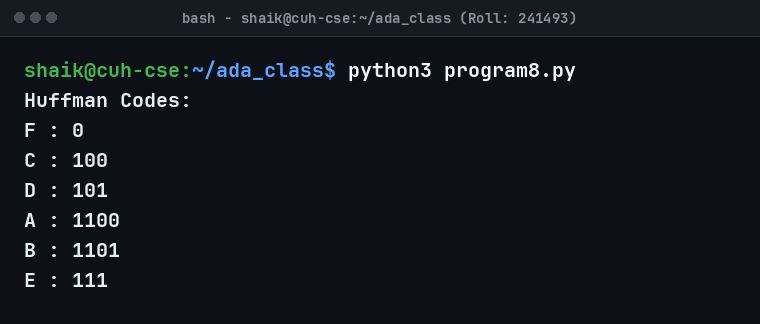
\includegraphics[width=0.88\textwidth]{Images/output_screenshot8.png}
\end{center}

\subsection*{GitHub Scan Code}
\begin{center}
    \begin{minipage}{0.3\textwidth}
        \centering
        % Generates a 2.5cm high QR code directly linking to the code file
        \qrcode[height=3.5cm]{https://github.com/gytdrop/ada_class/blob/main/program8.py} \\[0.2cm]
        \scriptsize\ttfamily Scan to view source code 
    \end{minipage}
\end{center}


% Add a horizontal line that indicates the END of the program.
\vspace{1cm}
\begin{center}
    \rule{1\textwidth}{1pt} % Clean, centered 1pt thick horizontal line
\end{center}